\documentclass[../../main.tex]{subfiles}

\begin{document}

In der Einführung hast du eine Reihe von Beispielen für Mengen gesehen. Damit du dir Mengen besser vorstellen kannst, ist es von Vorteil, wenn du sie zeichnen kannst. Dann kannst du sie mit einem Bild verbinden, das du dir merken kannst. 

\parpic[r]{
    \tikz{
        \node at (0,0) {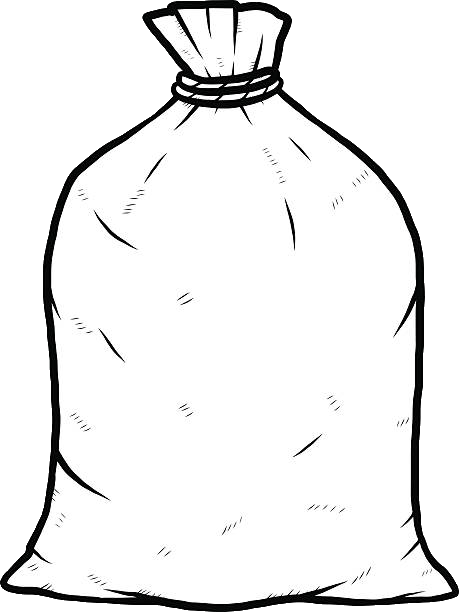
\includegraphics[height=3cm]{images/set_diagram.png}};
        \node[green!70!black] at (1.1,0.9) {\scriptsize grün};
        \node[blue] at (0,0.4) {\scriptsize blau};
        \node[red] at (0.3,-0.8) {\scriptsize rot};
        \node[yellow!70!black] at (-0.2,-0.1) {\scriptsize gelb};
        \draw[<-] (0.35,0.95) to[bend right] (0.8,1.45) node[above] {\scriptsize Grundfarben};
    }
}

Das haben wir in der Einführung auch schon gemacht. Du hast unter anderem die Menge der Grundfarben kennengelernt. Um sie dir vorstellen zu können, haben wir einen Behälter (nämlich den Sack, den du auf der rechten Seite siehst) gezeichnet. Wir stellen uns vor, dass alle Elemente unserer Menge sich innerhalb des Sacks befinden und alle anderen Objekte außerhalb. Deshalb befinden sich in der Zeichnung auch die drei Grundfarben rot, blau und gelb im Sack und die Farbe grün, die keine Grundfarbe ist, befindet sich außerhalb des Sacks.

Diese Darstellung ist hilfreich, aber eigentlich schon unnötig kompliziert. Eigentlich geht es ja gar nicht darum, ob wir einen Sack zeichnen oder vielleicht auch eine Keksdose, einen Karton oder welchen Behälter auch sonst. Wir können unsere Zeichnung daher auch vereinfachen.
\begin{example}[ex:first-venn-diagram]{}
    Wir haben die Menge der Grundfarben eben durch einen Behälter dargestellt, in dessen inneren sich die Grundfarben rot, blau und gelb befinden. Andere Objekte (zum Beispiel die Farbe grün) stellen wir uns außerhalb des Behälters vor.
    \parpic[r]{
        \begin{tikzpicture}
            \fill[grayset] (-1.5,0) circle (15mm);
            \node[label={[red]above:rot}, red] at (-1.5,0.7) {\textbullet};
            \node[label={[blue]above:blau}, blue] at (-2.5,0) {\textbullet};
            \node[label={[yellow!70!black]above:gelb}, yellow!70!black] at (-1.5,-1.1) {\textbullet};
            \node[label={[green!70!black]below:grün}, green!70!black] at (1.3,0.3) {\textbullet};
            \node (setName) at (1.2,1.5) {\textsc{Grundfarben}};
            \draw[->] (setName) to[bend left] (-0.3,0.5);
        \end{tikzpicture}
    }
    Das Bild auf der rechten Seite stellt genau die gleiche Menge dar, allerdings erfordert es nicht mehr ganz so viel künstlerisches Talent. Wir verzichten darauf, einen bestimmten Behälter zu zeichnen und deuten diesen stattdessen einfach durch einen Kreis an.

    \picskip{2}
    Der Kreis stellt also unsere Menge dar und die Elemente dieser Menge, die wir vorher in einen Behälter eingezeichnet haben, befinden sich nun im Kreis.
\end{example}

Im Beispiel haben wir den Behälter, den wir vorher gezeichnet haben, durch einen Kreis ersetzt. Ansonsten machen wir weiterhin alles wie vorher. Diagramme, in denen wir Mengen durch Kreise darstellen, heißen \textbf{Venn-Diagramme}. Sie sind nützlich, weil sie deutlich einfacher zu zeichnen sind als das Bild zu Beginn dieses Abschnitts.

Mithilfe von Venn-Diagrammen können wir auch übersichtlich mehrere Mengen auf einmal darstellen, indem wir die Kreise dafür einfach nebeneinander zeichnen.

\begin{example}[ex:venn-ohne-schnitt]{}
    \parpic[r]{
        \begin{tikzpicture}
            \fill[grayset] (-1.5,0) circle (15mm);
            \node[label={[red]above:rot}, red] at (-1.5,0.7) {\textbullet};
            \node[label={[blue]above:blau}, blue] at (-2.5,0) {\textbullet};
            \node[label={[yellow!70!black]above:gelb}, yellow!70!black] at (-1.5,-1.1) {\textbullet};
            \node (setName) at (1.2,1.5) {\textsc{Grundfarben}};
            \draw[->] (setName) to[bend left] (-0.3,0.5);
            %
            \fill[grayset] (1.5,0) circle (6mm);
            \node[label={[green!70!black]above:grün}, green!70!black] at (1.5,-0.3) {\textbullet};
            \node (greenName) at (0.7,-1) {\textsc{Grün}};
            \draw[->] (greenName) to (1.1,-0.2);
        \end{tikzpicture}
    }

    In Beispiel \ref{ex:first-venn-diagram} haben wir die Farbe \emph{grün}, die keine Grundfarbe ist, neben die Menge der Grundfarben gezeichnet. Damit sie nicht so alleine steht, erschaffen wir auch für die Farbe grün eine Menge
    \[\textsc{Grün}=\{\text{grün}\},\]
    die nur aus der Farbe grün besteht. Diese neue Menge können wir ganz einfach neben die Menge der Grundfarben zeichnen, die wir ja bereits kennen. Das entsprechende Venn-Diagramm sieht dann so aus wie wir es rechts gezeichnet haben.
\end{example}

\begin{example}[ex:venn-mit-schnitt]{}
    \parpic[r]{
        \begin{tikzpicture}
            \fill[grayset] (-1.5,0) circle (15mm);
            \fill[grayset] (0,0) circle (15mm);
            \draw (-1.5,0) circle (15mm);
            \node[label={[red]above:rot}, red] at (-1.5,0.7) {\textbullet};
            \node[label={[blue]above:blau}, blue] at (-2.5,0) {\textbullet};
            \node[label={[yellow!70!black]above:gelb}, yellow!70!black] at (-0.75,-0.3) {\textbullet};
            %\node (setName) at (1.2,1.5) {\textsc{Grundfarben}};
            %\draw[->] (setName) to[bend left] (-0.3,0.5);
            \node[label={[green!70!black]above:grün}, green!70!black] at (0.4,-0.8) {\textbullet};
            \node[label={[orange]above:orange}, orange] at (0.6,0.3) {\textbullet};
            %\node (greenName) at (0.7,-1) {\textsc{Mischfarben}};
            %\draw[->] (greenName) to (1.1,-0.2);
        \end{tikzpicture}
    }

    Wenn wir zwei Grundfarben mit einander mischen, dann erhalten wir eine neue Farbe. Mischen wir gelb mit gelb, dann haben wir natürlich immer noch gelb. Gelb und rot ergeben orange und gelb und blau ergeben grün. Wir können also eine der drei Mischfarben gelb, grün oder orange bekommen, wenn wir eine Grundfarbe mit gelb mischen.
    \[\textsc{Mischfarben}=\{\text{gelb},\text{grün},\text{orange}\}\]
    In diesem Fall haben unsere beiden Mengen ein gemeinsames Element: Die Farbe gelb ist sowohl eine Grundfarbe als auch in unserer neuen Menge \textsc{Mischfarben} enthalten. Du siehst deshalb rechts im Venn-Diagramm, dass die beiden Kreise sich überlappen. In der Mitte ist die Farbe gelb eingezeichnet, weil sie auf diese Weise in beiden Kreisen gleichzeitig liegt.
\end{example}

\parpic[r]{
    \begin{tikzpicture}[scale=0.6]
        \fill[grayset] (-1.5,0) circle (15mm);
        \fill[grayset] (0,0) circle (15mm);
        \fill[grayset] (-0.75,1.5) circle (15mm);
        \draw (-1.5,0) circle (15mm);
        \draw (0,0) circle (15mm);
        \draw (-0.75,1.5) circle (15mm);
    \end{tikzpicture}
}
Wenn wir zwei Mengen nebeneinander zeichnen, müssen wir die Kreise manchmal so zeichnen, dass sie sich überlappen. Auf diese Weise können wir dann auch Objekte einzeichnen, die sich in beiden Mengen gleichzeitig befinden.

Auf die gleiche Weise können wir auch drei Mengen gemeinsam in einem Diagramm darstellen. Das haben wir im Bild rechts gemacht. Ganz in der Mitte können wir Elemente einzeichnen, die sich in allen drei Mengen gleichzeitig befinden. Daneben gibt es Bereiche für Objekte, die sich in zwei Mengen, jedoch nicht in der dritten befinden. Mithilfe eines Venn-Diagramms siehst du also direkt auf einen Blick, welches eingezeichnete Objekt sich in welchen Mengen befindet.

Auf Dauer ist es anstrengend, immer darüber zu sprechen, dass ein Objekt sich in einer Menge $A$ und in einer Menge $B$ befindet, aber nicht in einer Menge $C$. Solche Sätze sind lang und unübersichtlich. Deshalb gibt es für die verschiedenen Bereiche in den Venn-Diagrammen, die wir gerade gesehen haben, Namen. Diese gehen wir nun nacheinander durch.

\parpic[r]{
    \begin{tikzpicture}
        \fill[black!10] (-1.5,0) circle (15mm);
        \fill[black!10] (0,0) circle (15mm);
        \fill[blue!20] ($(-1.5,0) + (60:1.5)$) arc [start angle=60, end angle=-60, radius=1.5] arc [start angle=240, end angle=120, radius=1.5] -- cycle;
        \draw (-1.5,0) circle (15mm);
        \draw (0,0) circle (15mm);
        \node at (-2, 0) {$A$};
        \node at (0.5, 0) {$B$};
        \node at (-0.75, 0) {$A\cap B$};
    \end{tikzpicture}
}
Wenn sich ein Objekt sowohl in einer Menge $A$ als auch in einer Menge $B$ befindet, dann zeichnen wir es im Bereich in der Mitte des Diagramms ein, der zu beiden Kreisen gehört. Dieser Bereich ist rechts blau markiert. Diesen Bereich nennen wir den \textbf{Schnitt} der Mengen $A$ und $B$. Für den Schnitt von $A$ und $B$ gibt es auch ein Symbol, nämlich $A\cap B$. Das Symbol für den Schnitt erinnert an das \emph{und}, das du aus dem Kapitel über \emph{Aussagenlogik} kennst. Alle Objekte, die sich sowohl in der Menge $A$ als auch in der Menge $B$ befinden, gehören also zum \emph{Schnitt} von $A$ und $B$.

Wir können den Schnitt zweier Mengen mithilfe der impliziten Schreibweise für Mengen, die du in der Einführung gesehen hast, wie folgt aufschreiben:
\[A\cap B=\{x~|~x\in A~\text{und}~x\in B\}\]
\begin{example}{}
    Der Schnitt der Menge \textsc{Grundfarben} und der Menge \textsc{Mischfarben} aus Beispiel \ref{ex:venn-mit-schnitt} enthält nur die Farbe gelb, denn dies ist die einzige Farbe, die sowohl zu den Grundfarben als auch zu den Mischfarben gehört. Es gilt also
    \[\textsc{Grundfarben}\cap\textsc{Mischfarben}=\{\text{gelb}\}.\]
\end{example}

\parpic[r]{
    \begin{tikzpicture}
        \fill[black!10] (-1.5,0) circle (15mm);
        \fill[black!10] (0,0) circle (15mm);
        \fill[blue!20] ($(-1.5,0) + (60:1.5)$) arc [start angle=60, end angle=300, radius=1.5] arc [start angle=-120, end angle=120, radius=1.5] -- cycle;
        \draw (-1.5,0) circle (15mm);
        \draw (0,0) circle (15mm);
        \node at (-2, 0) {$A$};
        \node at (0.5, 0) {$B$};
        \node at (-0.75, -1.75) {$A\cup B$};
    \end{tikzpicture}
}
Jedes Objekt, das wir im Venn-Diagramm in irgendeinem der Bereiche in den Kreisen einzeichnen, muss sich dafür zumindest in einer der Mengen $A$ oder $B$ befinden. Ein Objekt, das zumindest in einer der Mengen enthalten ist, zeichnen wir irgendwo im Bereich ein, der rechts blau markiert ist. Dieser Bereich heißt die \textbf{Vereinigung} der Mengen $A$ und $B$. Die Vereinigung können wir auch als $A\cup B$ schreiben. Das Symbol für die Vereinigung erinnert an das \emph{oder} aus der Aussagenlogik. Jedes Objekt, das zumindest in einer der Mengen $A$ oder $B$ enthalten ist, gehört also zur \emph{Vereinigung} von $A$ und $B$.

Ähnlich wie den Schnitt lässt sich auch die Vereinigung mit der impliziten Mengenschreibweise aufschreiben:
\[A\cup B=\{x~|~x\in A~\text{oder}~x\in B\}\]

\begin{example}{}
    Wenn wir alle Farben aufschreiben, die zur Menge \textsc{Grundfarben} oder zur Menge \textsc{Mischfarben} gehören, dann erhalten wir die Vereinigung
    \[\textsc{Grundfarben}\cup\textsc{Mischfarben}=\{\text{gelb},\text{rot},\text{blau},\text{grün},\text{orange}\}\]
    dieser beiden Mengen.
\end{example}

\parpic[r]{
    \begin{tikzpicture}
        \fill[black!10] (-1.5,0) circle (15mm);
        \fill[black!10] (0,0) circle (15mm);
        \fill[blue!20] ($(-1.5,0) + (60:1.5)$) arc [start angle=60, end angle=300, radius=1.5] arc [start angle=240, end angle=120, radius=1.5] -- cycle;
        \draw (-1.5,0) circle (15mm);
        \draw (0,0) circle (15mm);
        \node at (-2, 0) {$A$};
        \node at (0.5, 0) {$B$};
        \node (label) at (-0.75, -1.75) {$A\setminus B$};
        \draw[->] (label.west) to[bend left] (-1.8,-1.2);
    \end{tikzpicture}
}
Schließlich gibt es noch die Objekte, die nur zu einer der beiden Mengen gehören. Diese zeischnen wir zwar in die Mengen im Diagramm ein, aber nicht in die Mitte. Solche Objekte landen also zum Beispiel im blau eingezeichneten Bereich. Dort befinden sich alle Objekte, die zwar zu $A$ gehören, jedoch nicht auch noch zur Menge $B$ (sonst würden wir sie ja in die Mitte zeichnen). Dieser Bereich heißt die \textbf{Verminderung} von $A$ um $B$.

Anschaulich nimmst du also die Menge $A$ und entfernst alle Elemente, die auch in $B$ vorkommen. Du hast die Anzahl der Elemente von $A$ dadurch (in der Regel) \emph{vermindert}.

Die Schreibweise für die Verminderung von $A$ um $B$ ist $A\setminus B$, also ist
\[A\setminus B=\{x~|~x\in A~\text{und}~x\notin B\}.\]

\begin{example}{}
    Wenn wir aus der Menge der Grundfarben alle Farben entfernen, die in der Menge \textsc{Mischfarben} enthalten sind, dann erhalten wir
    \[\textsc{Grundfarben}\setminus\textsc{Mischfarben}=\{\text{rot},\text{blau}\}\]
    also die Verminderung von \textsc{Grundfarben} um \textsc{Mischfarben}. Die Farbe \emph{gelb} ist nicht in dieser neuen Menge enthalten, denn wir mussten sie entfernen, weil sie eine Mischfarbe ist.
\end{example}

Oft ist es auch hilfreich, einen Namen für diejenigen Elemente zu haben, die \emph{nicht} zu einer Menge gehören, die wir untersuchen. Zum Beispiel können wir, wenn wir die Menge $\textsc{Grün}=\{\text{grün}\}$ kennen, die nur die Farbe grün enthält, auch die Menge aufschreiben, die alle Farben \emph{außer} grün enthält:
\[\textsc{NichtGrün}=\{x\mid x\notin\textsc{Grün}\}\]
Die Menge, die alle Objekte enthält, die \emph{nicht} in einer anderen Menge $A$ enthalten sind, heißt das \textbf{Komplement} von $A$. Wir notieren das Komplement einer Menge, indem wir einen Strich über den Namen zeichnen. Zum Beispiel schreiben wir $\overline{A}$ für das Komplement von $A$. Es ist also
\[\overline{A}=\{x~|~x\notin M\}\]

\begin{example}{}
    Die Menge \textsc{NichtGrün}, die wir gerade definiert haben, enthält genau die Elemente, die nicht in der Menge \textsc{Grün} enthalten sind. Es gilt also
    \[\textsc{NichtGrün}=\{x\mid x\notin\textsc{Grün}\}=\overline{\textsc{Grün}}.\]
    Das heißt, \textsc{NichtGrün} ist das \emph{Komplement} der Menge \textsc{Grün}.
\end{example}

\begin{definition}{Vereinigung, Schnitt, Verminderung und Komplement}
    Seien $M$ und $N$ Mengen. Wir nennen
    \begin{itemize}
        \item $M\cup N\defas\{x~|~x\in M~\text{oder}~x\in N\}$ die \textbf{Vereinigung} von $M$ und $N$.
        \item $M\cap N\defas\{x~|~x\in M~\text{und}~x\in N\}$ den \textbf{Schnitt} von $M$ und $N$.
        \item $M\setminus N\defas\{x~|~x\in M~\text{und}~x\notin N\}$ die \textbf{Verminderung} von $M$ um $N$.
        \item $\overline{M}\defas\{x~|~x\notin M\}$ das \textbf{Komplement} von $M$.
    \end{itemize}
\end{definition}

\begin{nutshell}{Mengendiagramme}
    Mengen können effizient in \textbf{Venn-Diagrammen} dargestellt werden, indem du für jede Menge einen Kreis zeichnest, der die Elemente dieser Menge enthält. Objekte, die nicht zur Menge gehören, stellt man sich außerhalb des Kreises vor.

    Haben die Mengen gemeinsame Elemente, dann überlappen sich die Kreise. Die Bereiche im Venn-Diagramm, in denen sich ein Objekt abhängig davon befindet, ob es in einer, keiner oder mehreren gezeichneten Mengen enthalten ist, haben die folgenden Namen:
    \begin{multicols}{3}
        \begin{tikzpicture}[scale=0.8]
            \fill[black!10] (-1.5,0) circle (15mm);
            \fill[black!10] (0,0) circle (15mm);
            \fill[blue!20] ($(-1.5,0) + (60:1.5)$) arc [start angle=60, end angle=-60, radius=1.5] arc [start angle=240, end angle=120, radius=1.5] -- cycle;
            \draw (-1.5,0) circle (15mm);
            \draw (0,0) circle (15mm);
            \node at (-2, 0) {$A$};
            \node at (0.5, 0) {$B$};
            \node at (-0.75, 0) {$A\cap B$};
            \node at (-0.75, -1.75) {$A\cap B$};
        \end{tikzpicture}
        \begin{tikzpicture}[scale=0.8]
            \fill[black!10] (-1.5,0) circle (15mm);
            \fill[black!10] (0,0) circle (15mm);
            \fill[blue!20] ($(-1.5,0) + (60:1.5)$) arc [start angle=60, end angle=300, radius=1.5] arc [start angle=-120, end angle=120, radius=1.5] -- cycle;
            \draw (-1.5,0) circle (15mm);
            \draw (0,0) circle (15mm);
            \node at (-2, 0) {$A$};
            \node at (0.5, 0) {$B$};
            \node at (-0.75, -1.75) {$A\cup B$};
        \end{tikzpicture}
        \begin{tikzpicture}[scale=0.8]
            \fill[black!10] (-1.5,0) circle (15mm);
            \fill[black!10] (0,0) circle (15mm);
            \fill[blue!20] ($(-1.5,0) + (60:1.5)$) arc [start angle=60, end angle=300, radius=1.5] arc [start angle=240, end angle=120, radius=1.5] -- cycle;
            \draw (-1.5,0) circle (15mm);
            \draw (0,0) circle (15mm);
            \node at (-2, 0) {$A$};
            \node at (0.5, 0) {$B$};
            \node (label) at (-0.75, -1.75) {$A\setminus B$};
            \draw[->] (label.west) to[bend left] (-1.8,-1.2);
        \end{tikzpicture}
    \end{multicols}
    \begin{itemize}
        \item $M\cup N\defas\{x~|~x\in M~\text{oder}~x\in N\}$ die \textbf{Vereinigung} von $M$ und $N$.
        \item $M\cap N\defas\{x~|~x\in M~\text{und}~x\in N\}$ den \textbf{Schnitt} von $M$ und $N$.
        \item $M\setminus N\defas\{x~|~x\in M~\text{und}~x\not\in N\}$ die \textbf{Verminderung} von $M$ um $N$.
        \item $\overline{M}\defas\{x~|~x\not\in M\}$ das \textbf{Komplement} von $M$.
    \end{itemize}
\end{nutshell}

\end{document}